\documentclass[tikz, border=50pt]{standalone}

\usepackage{tikz}
\usepackage{medl_colors}
\usepackage{amsmath,xstring}
\usepackage{ifthen}
\usepackage{moresize}
\usetikzlibrary{shapes.multipart, shapes.geometric, arrows.meta}
\usetikzlibrary{matrix, calc, positioning,fit, backgrounds}
\begin {document}

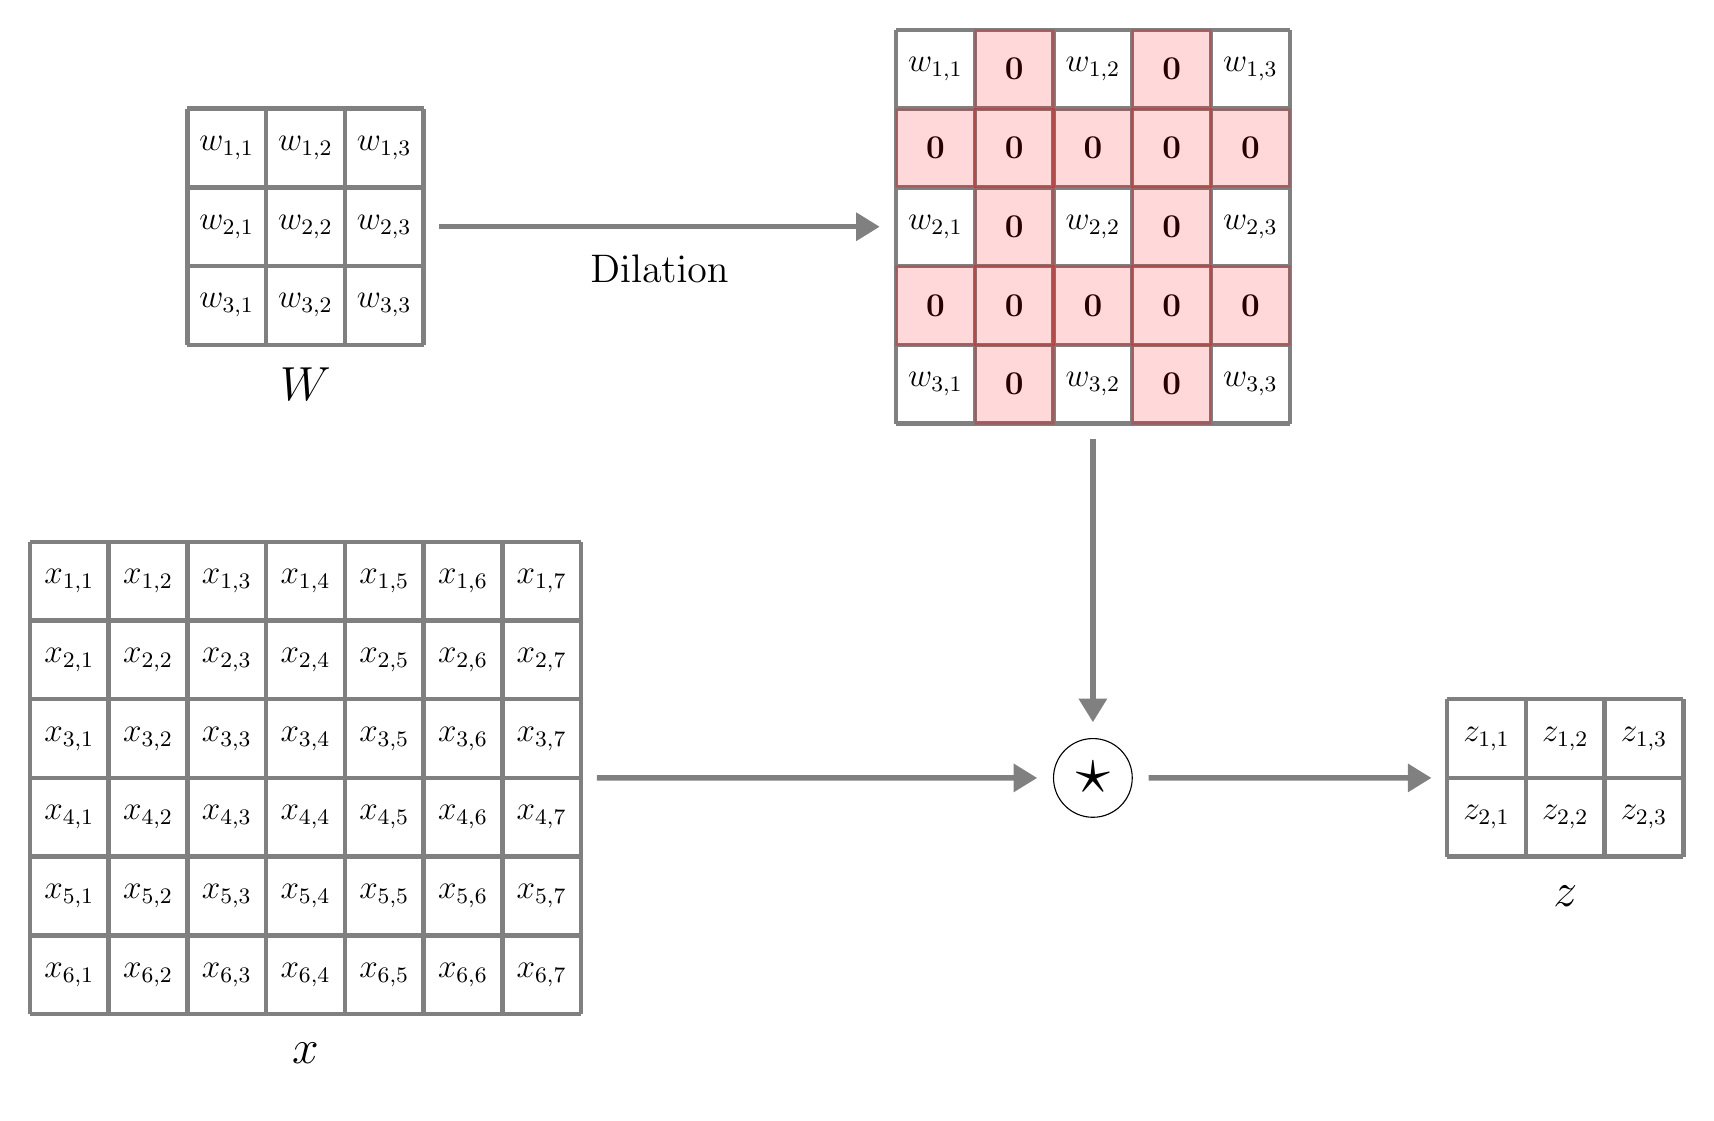
\begin{tikzpicture}[every node/.style={minimum size=1cm},on grid]

\begin{scope}

\newcommand\slantarray[7]{
    \draw[#6, ultra thick] (#1,#2) grid[step=1] (#1+#3, #2-#4) ;
    \foreach \i in {1,...,#3}{
        \foreach \j in {1,...,#4}{
            \IfEq{#7}{2}
            {
                \ifthenelse{\j=2 \OR \i=2 \OR \j=4 \OR \i=4 }
                {
                    \node (node-#7\i\j) at (#1+\i-.5, #2-\j+.5) {\large $\mathbf{0}$};
                    \node[rectangle, thick, minimum size=1cm, draw=red, fill=red, opacity=0.15] at (#1+\i-.5,#2+-\j+.5){};   
                }
                {
                     \node (node-#7\i\j) at (#1+\i-.5, #2-\j+.5) {};  
                }
            }
            {
                \node (node-#7\i\j) at (#1+\i-.5, #2-\j+.5) {\large $#5_{\j,\i}$};
            }
            
        }
    }

}

    \begin{scope}[yshift=.5cm]
        \slantarray{2}{2}{3}{3}{w}{black!50}{1};
        \slantarray{11}{3}{5}{5}{w}{black!50}{2};
    \end{scope}
    \slantarray{0}{-3}{7}{6}{x}{black!50}{3};
    \slantarray{18}{-5}{3}{2}{z}{black!50}{4};

 \foreach \i in {1,2,3}{
        \foreach \j in {1,2,3}{
            \node[] at (9.5+\i*2, 5-\j*2) {\large $w_{\j,\i}$};
        }
}
\node at (3.5,-1) {\LARGE $W$};
\node at (3.5,-9.5) {\LARGE $x$};
\node at (19.5,-7.5) {\LARGE $z$};
\node [draw, circle] at (13.5,-6) (circle) {\Huge $\star$};

\draw[-Triangle, draw=black!50, line width=.7mm] (node-132)+(7mm,-0mm) -- ([xshift=-2mm, yshift=0mm]node-213.west) node[pos=.5, below] {\Large Dilation};
\draw[-Triangle, draw=black!50, line width=.7mm] (node-373)+(7mm,-5mm) -- ([xshift=-2mm]circle.west) {};
\draw[-Triangle, draw=black!50, line width=.7mm] (node-235)+(0mm,-7mm) -- ([yshift=2mm]circle.north) {};
\draw[Triangle-, draw=black!50, thick, line width=.7mm] (node-411)+(-7mm, -5mm) -- ([xshift=2mm]circle.east) {};


\end{scope}
\end{tikzpicture}
\end{document}